\documentclass{article}
\usepackage[utf8]{inputenc}
\usepackage[dvipsnames]{xcolor}
\usepackage{fullpage,amsmath,amssymb,graphicx,mathtools}
\usepackage[shortlabels]{enumitem}
\usepackage{amssymb,amsmath,amsfonts,bbm,epsf,graphicx,hyperref,pstricks,pgfplots,comment,color}
\usepackage[bottom]{footmisc}
\usepackage{todonotes}
\allowdisplaybreaks

\newif\ifsolutions
\newenvironment{labelledanswer}{{\bf Answer:} \sf }{}%                               
\newcommand{\answer}[2]
{{
\ifsolutions
\begin{labelledanswer}
\color{red} 
#2
\end{labelledanswer}
\else
#1
\fi
}}
\solutionstrue

\def\nexp{n}
\def\di{d}
\def\fm{p}

\title{CS229 Final Exam - Summer 2020}
\date{Aug 14 2020 7am PDT - Aug 15 2020 7am PDT}

\begin{document}

\maketitle

 This exam is open-notes and open-internet. However, any and all forms of online or offline discussion is prohibited (for instance, posting questions on StackExchange is not permitted). We expect the exam to be completable in roughly 3 hours, but are giving you a 24-hour submission window to accommodate various time zones and upload speeds onto Gradescope. Good luck!

\section*{[0 points] The Stanford University Honor Code}

At the top of your solution file, please write/type the following Honor Code statement and attest it (i.e. sign or print your name below it), thereby implying your consent to follow the code:

``\textit{I attest that I have not given or received aid in this examination, and that
I have done my share and taken an active part in seeing to it that others
as well as myself uphold the spirit and letter of the Honor Code.}''

\textbf{Submissions without the attested Honor Code statement will NOT be graded.}

``\textit{I attest that I have not given or received aid in this examination, and that
I have done my share and taken an active part in seeing to it that others
as well as myself uphold the spirit and letter of the Honor Code.}''\\

Anh Vu L. Nguyen

\clearpage

\section{[10 points] True or False}

Each question is worth 1 point. Provide a short justification (one or two lines) for each answer. There will be no negative points, but answers without justification will not receive credit.

\bigskip

\noindent For questions 1-3, consider a binary classification task where we have $n$ training examples, $x^{(i)} \in \mathbb{R}^d$, and hypothesis $h_\theta(x)$ is parameterized by $\theta$. 

\begin{enumerate}

\item \textbf{True or False}. Removing half the training data will increase variance.

\answer{}{True, this should mean that the model will have less to work with for prediction. The test prediction will likely be larger than before, indicating incrase variance.}

\item \textbf{True or False}. Removing half of the features of $x$ will increase bias.

\answer{}{True, this would increase bias since it forces the model to assume more with less information available.}

\item \textbf{True or False}. Removing half of the features of $x$ will increase variance.

\answer{}{}

\item \textbf{True or False}. Adding a constant to the arguments of Radial Basis Function (RBF) kernel will not change the value of the kernel.

\answer{}{}

\item \textbf{True or False}. The following probability density function parameterized by $\theta$ belongs to the exponential family.
\begin{align}
f(x;\theta) = \frac{\theta^x}{2\pi x^3}e^{-\theta}
\end{align}

\answer{}{}

\item \textbf{True or False}. When training a neural network, it is a good practice to initialize all weights to $0$.

\answer{}{}

\item \textbf{True or False}. There is a unique solution to $k$-means clustering regardless of how we initialize the $k$ centers. 

\answer{}{}

\end{enumerate}

\noindent For questions 8-10, suppose we train a SVM classifier to perform binary classification using hinge loss, i.e. 
\begin{align}
    L(y_i) = \max\{0, 1 - y_i (w^T x_i + b)\} 
\end{align}

\begin{enumerate}

\setcounter{enumi}{7}

\item \textbf{True or False}. Adding a regularization term to the loss function can change the decision boundary.

\answer{}{}

\item \textbf{True or False}. Scaling each $x_i$ by constant $c$ can change the decision boundary.

\answer{}{}

\item \textbf{True or False}. Removing all data points that are not support vectors (i.e., their distance from the decision boundary is greater than $1$) can change the decision boundary.

\answer{}{}

\end{enumerate}

\clearpage

\section{[10 points] Short Answers}

Each question is worth 2 points. Provide a short justification (one or two lines) for each answer.

\begin{enumerate}

\item \textbf{Short Answer}. 
What 3 components can Mean Squared Error be decomposed into? Which component can be reduced by using a larger training set? Which component can be reduced by adding another hidden layer in a neural net? Which component can be reduced by decreasing the dimension of parameter $\theta$?

\answer{}{}

\item \textbf{Short Answer}. 
How many parameters are necessary to specify a \emph{Bernoulli Event Model} Naive Bayes classifier with $c$ classes and vocabulary size $v$? Express your answer in terms of $c$ and $v$.

\answer{}{We would need $v\times c$ parameters in total.}

\item \textbf{Short Answer}.
Suppose we train a neural network to classify 16 x 16 pixel images into 4 classes. We flatten each image into a vector, and feed the images into a 3-layer neural net with 10 neurons in the first hidden layer, 6 neurons in the second hidden layer, and apply softmax loss at the output layer. How many parameters does this model have? (Don't forget to include biases!)

\answer{}{}

\item \textbf{Short Answer}.
Consider a Markov Decision Process (MDP) defined as $(S, A, \{P_{sa}\}, \gamma, R)$, where $S$ is a finite set of $m$ states, $A$ is a finite set of $n$ actions, $\{P_{sa}\}$ are the transition probabilities, $\gamma$ is the discount factor, and $R$ is the reward function.
How many distinct deterministic policies $\pi:S\to A$ can be defined for this MDP?

\answer{}{}

\item \textbf{Short Answer}. Suppose we want to minimize a loss function parameterized by $\theta \in \mathbb{R}^d$, where $x \in \mathbb{R}^d$, $y \in \{-1, 1\}$, $z = y \theta^T x$, and the current value of z is -1.5. Which of the following loss functions would gradient descent fail to decrease, regardless of step size?
    \begin{enumerate}
        \item zero-one loss: $\varphi(z) = 1\{z \le 0\}$
        \item exponential loss: $\varphi(z) = e^{-z}$
        \item hinge loss: $\varphi(z) = \max\{1-z, 0\}$
    \end{enumerate}
\answer{}{
(a) would not work here as the loss function is a straight line and does not have anything for gradient descent to work with. I found a good graphical plot for all these loss functions:

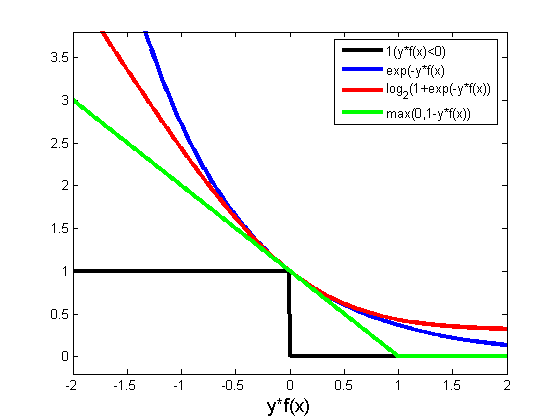
\includegraphics{loss_functions_q2_5.png}
}

\end{enumerate}

\clearpage

\section{[10 points] Theory \it{(Kernel Nearest Neighbor for Spam Classification)}}

In this problem, we will revisit the spam classification problem with the Kernel method. 

Recall that in homework 2 we implemented a Multinomial Event Model Naive Bayes classifier. Now we are going to combine the kernel method with the  K-nearest neighbor classification model. For simplicity, we use $k=1$ in the following scenario: for an incoming email, we calculate its kernel distance with each email in the training set, and assign the incoming email the label of the closest neighbor\footnote{If $k > 1$, we instead use the majority vote from the $k$ nearest neighbors as the predicted label.}. The performance of the algorithm highly depends on the kernel we choose, and we are going to compare options in this question.  

Let $S_i = [s_1, s_2, \cdots, s_{N_i}]$ be a string sequence (i.e. an email). Vocabulary $V$ is the set of all strings observed in any $S_i$. For a given sequence $S_i$, let $g_n(S_i)$ denote the set of all $n$-grams of $S_i$. For example,
    $$
        g_2([\text{I, saw, a, saw, that, saw, a, saw} ]) = \{\text{I saw},\,\text{saw a},\,\text{a saw},\,\text{saw that},\,\text{that saw}\}
    $$
    Notice here our 2-gram function only extracts one copy of `saw a' and `a saw'. Furthermore, we can define a string comparison function: 
\[
    \delta(s_j, s_k) =
\begin{cases}
  1,& \text{if } s_j = s_k\ \text{(i.e. the two n-gram strings are the same)}\\
    0,& \text{otherwise.}
\end{cases}
\]

\begin{itemize}
    \item [(a)] [4 points] 
    We define a kernel function as:
    $$
    K_{V,n}(S_1, S_2) = \sum_{x\in g_n(S_1)} \sum_{z\in g_n(S_2)} \delta(x, z)
    $$
    
    Express the kernel function using an appropriate feature mapping $\phi(S_i)$.
    That is, define the feature mapping $\phi(S_i) \in \mathbb{R}^d$ such that $K_{V,n}(S_1, S_2) = \phi(S_1)^\top\phi(S_2)$.
    What is the dimension of the feature mapping space $d$ in terms of $n$ and $V$?
    
    \emph{Hint}: The description of $\phi(S_i)$ should be brief.
    
    \answer{}{}
    
    \item[(b)] [3 points] In reality, the vocabulary size is usually large. For example {\it WikiText-103}, which contains all articles extracted from Wikipedia, has a vocabulary size of 217,646. However, the frequency of words has a long tail distribution and some of the words rarely appear. We can replace those rare words with a designated ``unknown token'' UNK to effectively reduce the vocabulary size. For example, if we restrict the vocabulary to $V'$ which only the has three tokens $\{ \text{I}, \text{saw}, \text{UNK}\}$, our previous example becomes: $S'_i = [\text{I, saw, UNK, saw, UNK, saw, UNK, saw}]$, and
    $$
        g_2(S'_i) = \{\text{I saw},\, \text{saw UNK}, \, \text{UNK saw}\}
    $$
    Let $V'$ be the reduced vocabulary, i.e. a subset of $\{V \cup \{\text{UNK})\}$.
    We define the kernel function for $V'$ as:
        $$
        K_{V', n}(S_1, S_2) = \sum_{x\in g_n(S'_1)} \sum_{z\in g_n(S'_2)} \delta(x, z)
    $$
    Is this still a valid kernel? If yes, express the kernel function using an appropriate feature mapping $\phi'(S_i)$ and state its relation with $\phi(S_i)$. If not, please give a counterexample.
    
    \answer{}{}
    
    \clearpage  
    
    \item[(c)] [2 points] Which of the following is true for any $V'$? Give a short explanation. 
    \begin{enumerate}
        \item [(A).] $K_{V, n}(S_1, S_2) \geq K_{V', n}(S_1, S_2)$
        \item [(B).] $K_{V, n}(S_1, S_2) \leq K_{V', n}(S_1, S_2)$
        \item [(C).] $K_{V, n}(S_1, S_2) > K_{V', n}(S_1, S_2)$
        \item [(D).] $K_{V, n}(S_1, S_2) < K_{V', n}(S_1, S_2)$
        \item [(E).] None of the above
    \end{enumerate}
    
    \answer{}{}
    
    \item[(d)] [1 points] Now we will apply this kernel to our spam classification problem. We hope that the nearest neighbor found through $K_{V', n}$, which is computationally more efficient, is the same as the nearest neighbor from the kernel space defined by $K_{V, n}$. 
    
    For any sequence $S_i$ in the training set $\mathcal{S}_{\text{train}}$, denote its ground truth label as $y(S_i)$. The Kernel Nearest Neighbor prediction for $S_t$ in the test set is:
    \[
        f_{V, n}(S_t) = y\left(\text{arg} \min_{S_i \in \mathcal{S}_{\text{train}}}  K_{V, n}(S_i, S_t)\right)\\
    \]
    We hope to observe:
    \[
        f_{V', n}(S_t) = f_{V, n}(S_t)  \tag{$\ast$} \label{eq:star}
    \]
    for any reduced vocabulary $V'$.
    
    Unfortunately, this is not true. We observe a trade-off between computational cost and accuracy: the smaller the vocabulary, the less computation is needed, but the more likely we do not find the true nearest neighbor. However, as long as the new vocabulary set $V'$ is not too small, this is still a good approximate classification model. 
    
    Give a concrete counterexample to the equation ($*$). You can choose any vocabularies $V, V'$, and $n$ for your example.
    
    \answer{}{}
    
\end{itemize} 

\clearpage 

\section{[10 points] Theory + Coding  \it{(The Poetic Scientist)}}

In this question, you will train a neural network to help write poetry. The goal is to find words that sound similar to each other. Weak supervision is one approach to learn how phonetically close or far two words are: your model will learn from and predict whether two inputs are similar or different sounding. Consider a two-layer network parameterized as follows:

\begin{align}
    h^{[1]}(x) &= W^{[1]}x + b^{[1]}\\
    a^{[1]}(x) &= \sigma(h^{[1]}(x))\\
    h^{[2]}(x) &= W^{[2]}a^{[1]}(x) + b^{[2]}
\end{align}

Our training examples will now consist of \textit{pairs} of inputs along with a label for whether the inputs are similar or dissimilar: $(x^{(i)}_1, x^{(i)}_2, y^{(i)}) \in \mathbb{R}^{d} \times \mathbb{R}^d \times \{-1, 1\}$ where $-1$ indicates a dissimilar pair and $1$ a similar pair. Consider the following loss:

\begin{align}
    \ell(x_1, x_2, y; W, b) = \log\left(1 + \exp(-y{h^{[2]}(x_1)}^\top h^{[2]}(x_2))\right)
\end{align}

\noindent \text{Theory:} [6 points]

\begin{itemize}
    \item [(a)] [1.5 points] Consider the loss for a single example. Write the expressions for $\frac{\partial \ell}{\partial h^{[2]}(x_1)},  \frac{\partial \ell}{\partial h^{[2]}(x_2)}$. 
    
    \answer{}{}
    
    \item [(b)] [1.5 points] Express $\frac{\partial \ell}{\partial W^{[2]}}$, $\frac{\partial \ell}{\partial b^{[2]}}$ in terms of $\frac{\partial \ell}{\partial h^{[2]}(x_1)}$ and $\frac{\partial \ell}{\partial h^{[2]}(x_2)}$ and $a^{[1]}(x_1), a^{[1]}(x_2)$.
    
    \answer{}{}
    
    \item [(c)] [1.5 points] Express $\frac{\partial \ell}{\partial h^{[1]}(x_1)}$, $\frac{\partial \ell}{\partial h^{[1]}(x_2)}$ in terms of model parameters and $\frac{\partial \ell}{\partial h^{[2]}(x_1)}, \frac{\partial \ell}{\partial h^{[2]}(x_2)}$.
    
    \answer{}{}
    
    \item [(d)] [1.5 points] Express $\frac{\partial \ell}{\partial W^{[1]}}$, $\frac{\partial \ell}{\partial b^{[1]}}$ in terms of $\frac{\partial \ell}{\partial h^{[1]}(x_1)}$, $\frac{\partial \ell}{\partial h^{[1]}(x_2)}$ and $x_1, x_2$.
    
    \answer{}{}
    
\end{itemize}

\noindent \text{Coding:} [4 points]

\begin{itemize}

    \item [(e)] 

Your friend suggests an alternative to your approach: A single layer, shared by both inputs $x_1^{(i)}$ and $x_2^{(i)}$, that outputs two vectors, $z_1^{(i)} \in \mathbb{R}^{25}$ and $z_2^{(i)} \in \mathbb{R}^{25}$, respectively. Each output represents the input's word embedding: a representation of the input as a point in a vector space that's conducive to further processing. We are interested in the distance $d^{(i)}$ between two embeddings $z_1^{(i)}$ and $z_2^{(i)}$. The weakly supervised labels $y^{(i)} \in \{0, 1\}$ where $0$ indicates a similar-sounding pair and $1$ a different-sounding one; $B$ is the batch size. 

Extract the zip file and run \texttt{conda env create -f environment.yml} from inside the extracted directory. This creates a Conda environment called \texttt{cs229-final}. Run \texttt{source activate cs229-final} to activate this environment. In \texttt{train.py}, please fill in the functions corresponding to (e), (f), (g), and include the 3 generated outputs in part (h). 
    
    \begin{enumerate}[(i)]
    \item Fill in the code for the \texttt{batch\_dot} function ($a \cdot b$ denotes the dot product):
    
    \begin{align}
    \mathrm{batch\_dot}(z_1, z_2) = \begin{bmatrix}
        z_1^{(1)} \cdot z_2^{(1)} \\
        \vdots \\
        z_1^{(i)} \cdot z_2^{(i)} \\
        \vdots \\
        z_1^{(B)} \cdot z_2^{(B)}
    \end{bmatrix} \in \mathbb{R}^{B}
    \end{align}
    \item Fill in the code for the \texttt{distance\_loss} function:
    
    \begin{align}
    \mathrm{distance\_loss}(y, d) = \frac{1}{B} \sum_{i = 1}^{B} \left[ (1 - y^{(i)}) \; (d^{(i)})^2 + y^{(i)} \; (1 - d^{(i)})^2 \right]
    \end{align}
    \item Use the following to fill in the code for the \texttt{accuracy} function:
    
    \begin{align}
    \hat{y}^{(i)} = \mathbbm{1}\{d^{(i)} > 0.5\} \\
    \mathrm{accuracy}(y, d) = \frac{1}{B} \sum_{i = 1}^{B} \mathbbm{1}\{ y^{(i)} = \hat{y}^{(i)} \}
    \end{align}
    \end{enumerate}

Run \texttt{train.py} and submit the 2 learning curve plots (loss vs epochs, accuracy vs epochs) along with the sample of embeddings projected onto a two-dimensional plot. As usual, pay attention to the documentation in the code and upload your code (\texttt{train.py}) to Gradescope. \textbf{Hint:} Dev accuracy at the end of training $\approx 0.71$.
    
\end{itemize}

\answer{}{}

\end{document}
